\section{Method}
\label{sec:method}

We cast paragraph-level context selection as a per-candidate scoring
problem, then study two combinations of six heterogeneous trust
signals: a naive uniform average and a small supervised logistic
regression. The end-to-end pipeline is summarized in
Figure~\ref{fig:fig-architecture}, and the signal taxonomy in
Figure~\ref{fig:fig-signal-taxonomy}.

\begin{figure}[t]
  \centering
  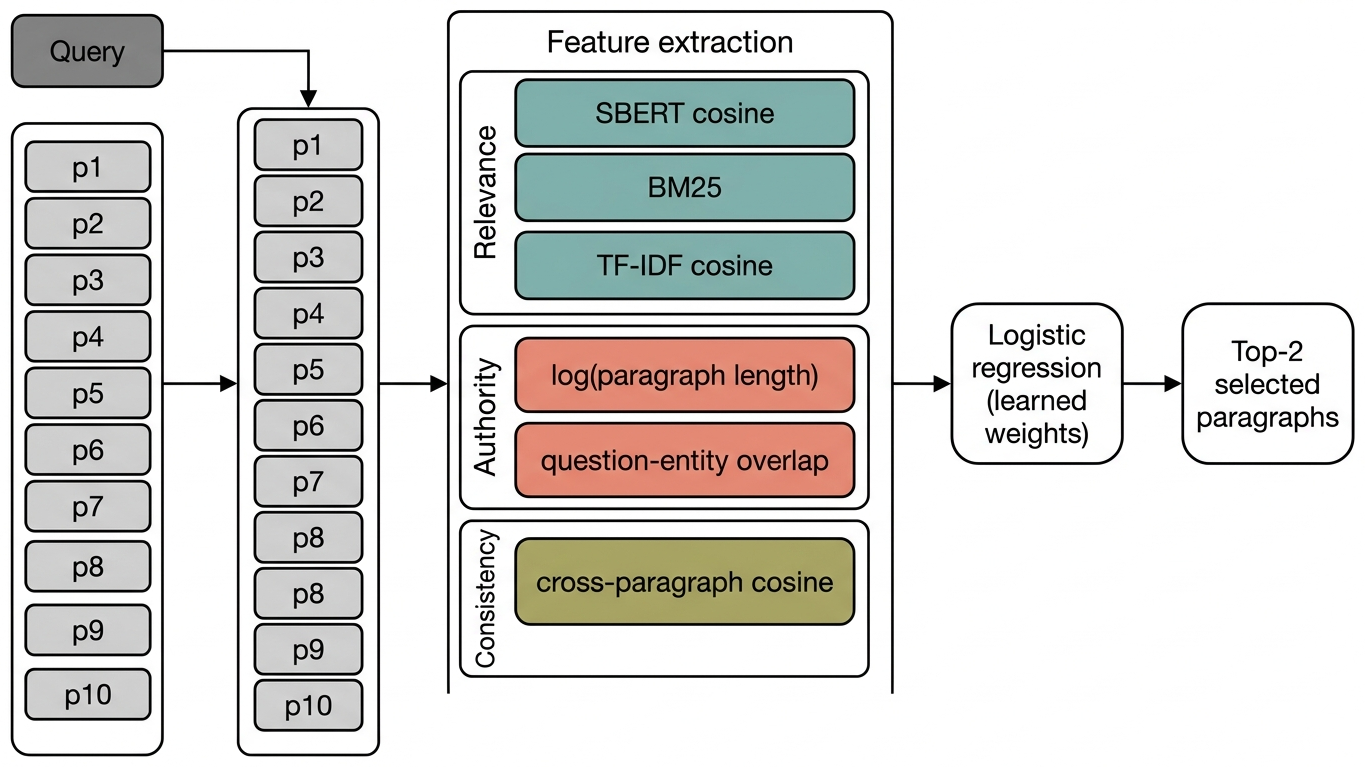
\includegraphics[width=0.95\linewidth]{figures/fig-architecture.png}
  \caption{Trust-aware paragraph selection. For each query, the ten
  candidate paragraphs are scored by six per-paragraph signals spanning
  relevance (SBERT, BM25, TF-IDF), authority proxies (log-length,
  question-entity overlap), and cross-paragraph consistency. A
  six-feature logistic regression combines the per-candidate feature
  vector into a scalar trust score; the top-2 paragraphs are selected.}
  \label{fig:fig-architecture}
\end{figure}

\subsection{Problem formulation}

Each example comprises a query $q$ and a pool of $n=10$ candidate
paragraphs $\mathcal{P}=\{p_1,\ldots,p_n\}$, of which two are
\emph{gold} supporting paragraphs labeled $y_i=1$ and eight are
\emph{distractors} with $y_i=0$. A trust scorer
$s : (q, p_i, \mathcal{P}) \mapsto \mathbb{R}$ returns a scalar per
candidate. Selection keeps the top-$K$ indices,
$\hat{\mathcal{S}} = \operatorname*{argtop}_K s(q, p_i, \mathcal{P})$,
with $K=2$.

\subsection{Trust signals}

We evaluate six per-candidate features, grouped by the trust dimension
each is intended to capture (Figure~\ref{fig:fig-signal-taxonomy}).

\begin{figure}[t]
  \centering
  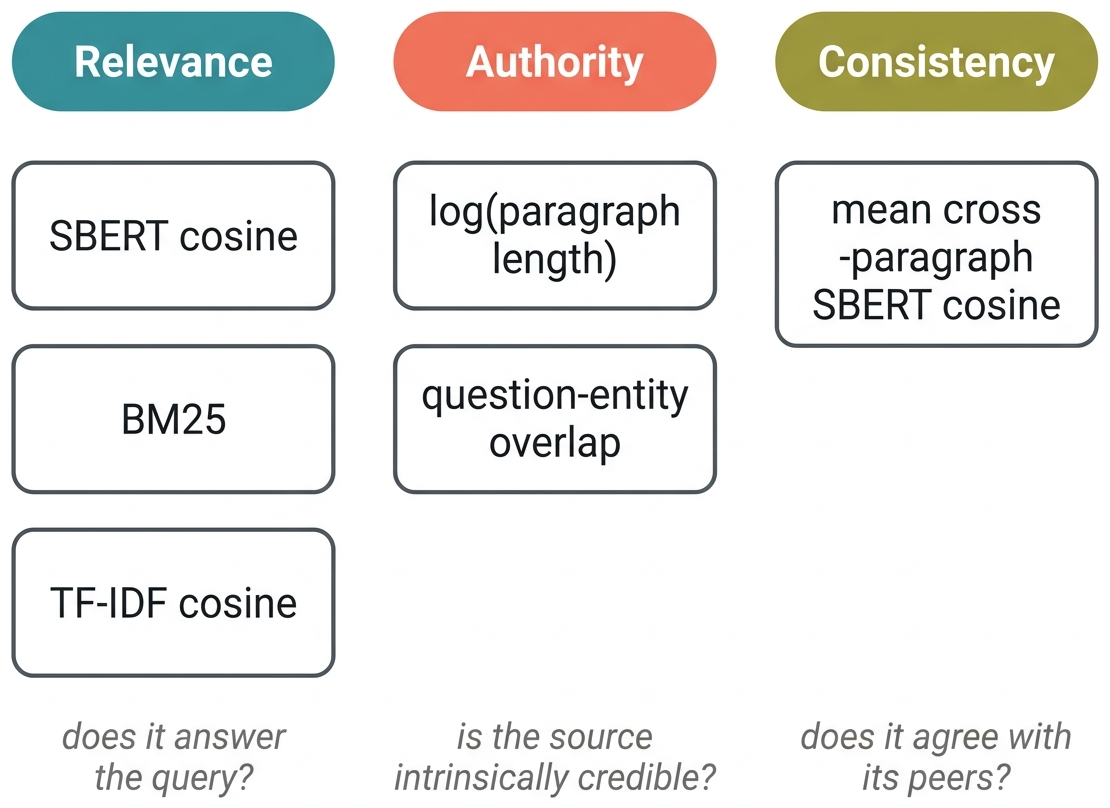
\includegraphics[width=0.85\linewidth]{figures/fig-signal-taxonomy.png}
  \caption{Taxonomy of trust signals. Relevance asks whether the
  paragraph answers the query; authority asks whether the paragraph is
  an intrinsically credible source; consistency asks whether the
  paragraph agrees with the rest of the candidate pool.}
  \label{fig:fig-signal-taxonomy}
\end{figure}

\textbf{Relevance.} How well does $p_i$ answer $q$? We use three
measures: (a) BM25 over bag-of-lowercased-tokens~\cite{robertson2009bm25};
(b) TF-IDF cosine between $q$ and $p_i$ using a vocabulary fit jointly
on $\{q\}\cup\mathcal{P}$; (c) cosine similarity between sentence
embeddings $\phi(q)$ and $\phi(p_i)$ from all-MiniLM-L6-v2, a compact
sentence-transformer~\cite{reimers2019sbert}.

\textbf{Authority.} How intrinsically credible is $p_i$, independent of
the query? We use two cheap proxies: (a) $\log(1+|p_i|_{\text{tok}})$,
encoding the assumption that a Wikipedia stub is typically shorter than
a well-developed article; (b) question-entity overlap,
$\lvert\mathcal{E}(q)\cap\mathcal{E}(p_i)\rvert / \lvert\mathcal{E}(q)\rvert$,
where $\mathcal{E}(\cdot)$ returns the set of capitalized $n$-grams
(regex \texttt{[A-Z][A-Za-z0-9]+(?:\textbackslash s+[A-Z][A-Za-z0-9]+)*})
and multi-digit numeric tokens (regex \texttt{\textbackslash d\{2,\}})
after filtering English stop words of length $< 3$. The overlap is a
lightweight stand-in for named-entity recognition that avoids an
external parser; we verified on 20 random examples that it recovers
most named entities a spaCy \texttt{en\_core\_web\_sm} tagger would
produce, at the cost of also capturing sentence-initial common nouns.

\textbf{Consistency.} How much does $p_i$ agree with the rest of the
candidate pool? We use the mean SBERT cosine to the other $n-1$
candidates:
\begin{align*}
\operatorname{cons}(p_i) \;=\; \tfrac{1}{n-1}\!\sum_{j \ne i} \cos\!\bigl(\phi(p_i),\phi(p_j)\bigr).
\end{align*}
A trust reading of this signal would be ``this claim is corroborated by
other sources''. A later section revisits whether that reading holds in
distractor-rich retrieval.

\subsection{TrustScore variants}

Both combinations first min-max normalize each signal across the
candidate pool of its own question, so that per-question score
distributions are comparable.

\textbf{TrustScore-Uniform (ablation).} The naive baseline averages
three normalized signals with equal weight:
\begin{align*}
s_{\text{uniform}}(p_i) \;=\; \tfrac{1}{3}\!\bigl(\tilde r_{\text{SBERT}}(p_i)\;+\;\tilde a_{\text{len}}(p_i)\;+\;\tilde c(p_i)\bigr),
\end{align*}
where $\tilde r_{\text{SBERT}}$ is normalized SBERT relevance,
$\tilde a_{\text{len}}$ is normalized log-length, and $\tilde c$ is
normalized cross-paragraph consistency. This encodes the intuition
``trustworthy equals relevant plus authoritative plus corroborated''
without checking whether each signal actually points toward gold.

\textbf{TrustScore-Learned (proposed).} We fit a logistic regression
$\sigma(\mathbf{w}^\top \mathbf{x}_i + b)$ over the six-dimensional
normalized feature vector
$\mathbf{x}_i = (\tilde r_{\text{SBERT}}, \tilde r_{\text{BM25}}, \tilde r_{\text{TFIDF}}, \tilde a_{\text{len}}, \tilde a_{\text{ent}}, \tilde c)$
with binary gold labels $y_i\in\{0,1\}$, using scikit-learn's implementation~\cite{pedregosa2011sklearn}
with $L_2$ regularization. The trust score is the predicted gold
probability,
$s_{\text{learned}}(p_i) = \sigma(\mathbf{w}^\top \mathbf{x}_i + b)$.

The classifier is refit from scratch for each random seed on a disjoint
training split of 100 questions. We deliberately keep both the feature
count (six) and the training budget (100 questions per seed) small, so
that any gain over single-signal baselines is attributable to signal
combination, not to classifier capacity. Per-seed refitting prevents
any test-split contamination between the training of the trust scorer
and the evaluation of the system.

\subsection{Selection}

At evaluation, for each test question we compute
$s(q, p_i, \mathcal{P})$ for every candidate and return the two
paragraphs with the highest score. The scorer is pointwise: no
cross-candidate attention, no re-ranking pass, no backtracking. This
keeps the architecture within the simplest regime in which a
trust-weighted selection can be studied, and isolates the effect of
signal combination from the effect of listwise learning.
